\documentclass[12pt]{article}
\usepackage[margin=1in]{geometry}
\usepackage{amsmath,amssymb,booktabs,tabularx,array,graphicx,setspace,float}
\usepackage[font=small,labelfont=bf]{caption}
\usepackage[hidelinks]{hyperref}
\usepackage{microtype}
\graphicspath{{results/figures/}}
\onehalfspacing
\setlength{\parskip}{5pt}
\setlength{\parindent}{0pt}
\setlength{\emergencystretch}{4em}
\newcommand{\R}{\mathbb{R}}
\title{\textbf{MECH 559 -- Individual Rotor Optimization Report}\\
\large Experimental-Envelope-Constrained Selection for a Quad-Tiltrotor UAV}
\author{Ashish Giri \quad Group 5 \quad VTOL Rotor Subsystem}
\date{November 2026}
\begin{document}
\maketitle
\begin{abstract}
This individual report develops and verifies a rotor subsystem optimization for a four-rotor tiltrotor UAV, emphasizing experimentally supportable aerodynamic predictions. A previous free-geometry blade-element/momentum-theory (BEMT) optimization was audited and rejected as the basis for hardware selection because its induced-flow solver silently clipped negative local aerodynamic loading. The replacement performs a discrete search over measured two-bladed APC propellers and optimizes hover and cruise rotational speeds by interpolating independently published thrust and power coefficients without extrapolating outside measured conditions. For a \emph{modified} 40-km, 20-m/s cruise mission with five minutes of hover and an illustrative 9.5-kg base aircraft mass (including the 5-kg payload but excluding propeller blades), an APC 18$\times$12E gives 278.3 Wh of rotor electrical energy at 3,890 RPM hover and 3,500 RPM cruise. It is a screening recommendation, not a certified final aircraft design. Under the proposal's official 40-km/20-min cruise requirement (33.3 m/s), the screened catalogue has no measured-domain feasible cruise-trim result. The difference is explicitly treated as a design finding rather than hidden by extrapolation.
\end{abstract}

\section*{1. PROBLEM STATEMENT}
The vehicle is a fixed four-rotor tiltrotor that must use the same propellers for static hover and forward-flight propulsion. The rotor subsystem contributes thrust, power, motor torque, aerodynamic installation area, and component mass to the coupled vehicle. Larger discs generally reduce ideal hover-induced power, whereas rotor mass, blade drag, mounting clearance and cruise advance ratio penalize excessive diameter or low-pitch designs. Rotor selection must therefore account for the entire mission, not hover power alone.

The project proposal states a 5-kg \emph{payload}, a 40-km sortie, five total minutes of hover, and 20 minutes of cruise. These requirements imply a mean cruise speed of $40{,}000/1{,}200=33.33$ m/s. Earlier rotor screens instead used 5 kg \emph{total takeoff mass}, 36 km at 20 m/s, and two minutes of hover. The two cases are not interchangeable. Since agreed aircraft takeoff mass, cruise drag and actual motor maps are not yet available, this report (i) formally checks the official speed against the available measured propeller envelope and (ii) investigates a clearly identified 40-km, 20-m/s alternative to quantify meaningful, data-backed energy and hardware-interface numbers.

The scientific aim is to obtain a credible rotor result with an honest range of validity. UIUC Volume 4 wind-tunnel data for APC Thin Electric propellers provide both static and axial-flow $C_T,C_P$ measurements. APC product specifications provide propeller-only masses. These are real published observations, not outputs from our aerodynamic optimizer. The design is rejected whenever the necessary forward-flight condition lies outside the measured advance-ratio/RPM domain. The study does not claim to prove flightworthiness or replace motor and battery integration.

\section*{2. DESIGN OPTIMIZATION PROBLEM FORMULATION}
\subsection*{2.1 Decision variables and justified model architecture}
The original exploratory formulation used five continuous variables $[R,c,\Omega_h,\Omega_c,\theta_{75}]$, with $N_b\in\{2,3,4\}$. That choice is well suited to a validated blade-section model, but the original implementation was not physically consistent in negative-loaded annuli and its assumed $C_l,C_d$ produced major measured-data errors. Reporting its optimum as experimentally accurate would therefore be unjustified. Instead, the \emph{experimental-envelope-constrained problem} uses a discrete catalogue choice $s$ (which fixes measured diameter, propeller pitch family, and $N_b=2$) and continuous $\Omega_h,\Omega_c$. All published catalogue candidates here are two-bladed. The reduction in design freedom is intentional: independent chord and continuous pitch variations cannot be supported by the available published data. The initial five-variable research formulation is preserved as a future design-space extension, not disguised as a completed validated model.

The principal candidates are APC 16$\times$12E, 18$\times$10E, 18$\times$12E, and 20$\times$10E. The first number is nominal diameter in inches and the second nominal pitch in inches per revolution; nominal pitch is \emph{not} a measured $\theta_{75}$. For a reference helical approximation only, the 18$\times$12 pitch corresponds to $\arctan[p/(2\pi(0.75R))]\simeq15.8^\circ$; this is not substituted for actual radial blade geometry. Catalogue masses were taken from APC's current product specifications and add no assumed motor or nacelle masses.

\subsection*{2.2 Data-grounded aerodynamic analysis}
With $n=\Omega/(2\pi)$ in revolutions/s, $D=2R$, air density $\rho$, and axial airspeed $V$, the experimentally defined coefficients are
\begin{equation}
J=\frac{V}{nD},\qquad C_T=\frac{T}{\rho n^2D^4},\qquad C_P=\frac{P_{\mathrm{sh}}}{\rho n^3D^5}.
\label{eq:coeff}
\end{equation}
For a candidate propeller, measured static $C_T$ and $C_P$ are shape-preserving interpolated in RPM. Forward-flight coefficients are interpolated first in $J$ within each recorded RPM curve and then linearly between adjacent measured RPM curves. \emph{Both bracketing RPM runs must cover the requested $J$.} Extrapolation in RPM, advance ratio, blade count or geometry is rejected. The derived shaft torque and propulsive efficiency are
\begin{equation}
Q=\frac{P_{\mathrm{sh}}}{\Omega},\qquad \eta_p=\frac{TV}{P_{\mathrm{sh}}}=\frac{JC_T}{C_P}.
\end{equation}
This is an interpolation-based measured-performance model, not a newly experimentally validated BEMT prediction. Interpolation at withheld points is used as a numerical accuracy audit and is not represented as independent physical validation of a new propeller.

\subsection*{2.3 Loads, objective, and constraints}
Let $N_r=4$, payload already be part of the specified base mass $m_b$, and let $m_p(s)$ be one measured propeller blade assembly mass. To avoid double counting motor mass, define $m_b$ as all other aircraft components and payload \emph{excluding only the four propellers}, so
\begin{equation}
m_{TO}=m_b+4m_p(s),\quad
T_{h,\mathrm{req}}=\frac{(1+\delta_{dl})m_{TO}g}{4},\quad
T_{c,\mathrm{req}}=\frac{D_c}{4}.
\label{eq:requirements}
\end{equation}
For phase times $t_h=300$ s and $t_c=L_c/V_c$, the component-level electrical-energy objective (Wh) is
\begin{equation}
\min_{s,\Omega_h,\Omega_c} E_r =
\frac{4}{3600\eta_d}\left[P_{h,\mathrm{sh}}(s,\Omega_h)t_h
+P_{c,\mathrm{sh}}(s,\Omega_c,V_c)\frac{L_c}{V_c}\right].
\label{eq:objective}
\end{equation}
The illustrative drive efficiency is $\eta_d=0.85$. Exact steady-flight trim is imposed at the \emph{same} speed used to compute torque and power:
\begin{equation}
T_h-T_{h,\mathrm{req}}=0,\qquad T_c-T_{c,\mathrm{req}}=0.
\end{equation}
The additional constraints are the specified 15\% measured hover thrust reserve, rotor installation clearance $D+\Delta_{clear}\le s_{mount}$, motor torque $Q_h,Q_c,Q_{reserve}\le Q_{max}$, tip Mach $M_{tip}\le M_{lim}$ and total electrical power (including reserve) $4P_{sh}/\eta_d\le P_{max}$. Only points inside the measured static and forward-flight domains are admissible. For the exploratory case, $m_b=9.5$ kg, $D_c=7$ N, $\delta_{dl}=0.05$, $s_{mount}=0.65$ m, $\Delta_{clear}=0.05$ m, $Q_{max}=1.5$ N m, $M_{lim}=0.65$, and $P_{max}=2400$ W. Apart from cited product masses and aerodynamic measurements, these limits are \emph{provisional system interfaces}, not agreed teammate specifications.

\begin{table}[H]
\centering\small
\caption{Functional-dependency structure of the rotor component optimization.}
\begin{tabularx}{\linewidth}{@{}p{0.26\linewidth}X X@{}}
\toprule
Function/analysis & Rotor decisions and model dependence & Supplied system parameters \\
\midrule
Hover thrust and shaft power & $s,\Omega_h;\ C_T,C_P$ static & $\rho,m_b,\delta_{dl}$ \\
Cruise thrust and shaft power & $s,\Omega_c;\ C_T,C_P(J,\mathrm{RPM})$ & $D_c,V_c,\rho$ \\
Mass-closure load & $s,\ m_p(s)$ & Payload, wing, motor and battery masses \\
Mission electrical energy & $P_{h,sh},P_{c,sh}$ & $t_h,L_c,V_c,\eta_d$ \\
Motor/installation constraints & $Q,\Omega,D$ and reserve trim & $Q_{max},P_{max},s_{mount},\Delta_{clear}$ \\
Data-domain feasibility & Candidate RPM and measured $J$ range & Availability of UIUC test measurements \\
\bottomrule
\end{tabularx}
\label{tab:dependency}
\end{table}

\subsection*{2.4 Well-posedness, model correction and numerical regularity}
The catalogue is finite, each RPM domain is bounded, and coefficients are continuous within retained data segments; therefore any feasible component candidate has a bounded objective. This does not imply the original five-variable BEMT formulation is globally convex. The old BEMT solver had replaced negative annular thrust and torque with zero in the induced-flow momentum update while retaining negative loads in its final integrals. A replacement diagnostic implements the \emph{signed} annular momentum equations
\begin{equation}
\frac{dT}{dr}=4\pi\rho Fr(V+v_i)v_i,\qquad
\frac{dQ}{dr}=4\pi\rho Fr^2(V+v_i)v_\theta,
\end{equation}
returning an invalid-regime flag when no physical low-induction branch exists instead of silently clipping loads. When reevaluated, the prior three-blade cruise operating point fails this domain check. Accordingly, the previously reported 138.10 Wh screening optimum is retired and is not used in any design recommendation.

For each catalogue candidate, the two continuous equality constraints have a 2-by-2 normalized local Jacobian. At the measured-domain 18$\times$12E alternative optimum its rank is 2 and its condition number is approximately 12.8, supporting local regularity. This first-order check does not prove a global optimum over propeller geometries outside the catalogue.

\section*{3. NUMERICAL OPTIMIZATION RESULTS}
\subsection*{3.1 Numerical method and starting points}
Four discrete two-blade candidates were enumerated. Within each candidate, hover and cruise thrust residuals were independently bracketed and solved with Brent's method on only those intervals where measured interpolation is defined. The resulting exactly trimmed RPM pair was supplied as the initial guess to a two-variable, equality-constrained SLSQP problem; candidate feasibility was checked independently against reserve, torque, tip-speed, installation and power limits. This ``root check + SQP'' architecture exposes solver errors instead of falsely regarding an unsuccessful search as proof of physical infeasibility. Candidate count and the measured input domain, rather than initial guesses, dominate this validated search.

For the 18$\times$12E solution SLSQP terminated after \textbf{one iteration, three function evaluations}, with maximum scaled trim residual $1.7\times10^{-12}$. Because the initial point was already an exact trim, this is \emph{not} evidence of a difficult five-dimensional nonlinear search; the important optimization is catalogue selection and documented comparison of experimentally available operating points. Independent root-solving gives the same 278.31 Wh result to numerical precision. Course concepts of active constraints, regularity and constrained numerical optimization are thus used in an appropriately limited role.

\subsection*{3.2 Two distinct mission cases and catalogue feasibility}
\begin{table}[H]
\centering\small
\caption{Mission conditions; official mission requirements are \emph{not} replaced by the slower alternative.}
\begin{tabularx}{\linewidth}{@{}lXX@{}}
\toprule
Input & Official project mission & Data-supported alternative \\
\midrule
Payload & 5 kg & 5 kg (included in base mass) \\
Cruise distance & 40 km & 40 km \\
Total hover & 5 min & 5 min \\
Cruise speed / duration & 33.33 m/s / 20 min & 20 m/s / 33.33 min \\
Takeoff-mass example & 9.5 kg base + propellers (assumed) & Same assumed base mass \\
Cruise drag & 7 N provisional for comparison & 7 N provisional \\
\bottomrule
\end{tabularx}
\end{table}
\begin{table}[H]
\centering\small
\caption{Experimental-envelope screening of four APC two-bladed candidates.}
\begin{tabularx}{\linewidth}{@{}lccXX@{}}
\toprule
Propeller & Diameter (m) & Prop mass (g) & 20-m/s alternative & 33.33-m/s official \\
\midrule
16$\times$12E & 0.406 & 51.9 & No measured-domain cruise trim & No measured-domain cruise trim \\
18$\times$10E & 0.457 & 72.9 & No measured-domain cruise trim & No measured-domain cruise trim \\
18$\times$12E & 0.457 & 74.0 & Feasible screening trim & No measured-domain cruise trim \\
20$\times$10E & 0.508 & 96.1 & No measured-domain cruise trim & No measured-domain cruise trim \\
\bottomrule
\end{tabularx}
\end{table}
Here ``no measured-domain cruise trim'' means \emph{the available tested RPM and advance-ratio ranges do not contain a verified matching operating point}; it does not prove that the actual propeller cannot produce sufficient thrust outside those conditions, nor that a different rotor family cannot meet the official mission. No out-of-range aerodynamic performance is invented.

\subsection*{3.3 Best data-supported alternative and engineering checks}
For the illustrative base mass of 9.5 kg, with four 74-g propellers, $m_{TO}\simeq9.796$ kg and required hover thrust is 25.226 N per rotor. The 18$\times$12E selected within the \emph{restricted} catalogue yields the following results:
\begin{table}[H]
\centering\small
\caption{APC 18$\times$12E measured-envelope operating conditions (alternative mission only).}
\begin{tabular}{@{}lrlr@{}}
\toprule
Quantity & Value & Quantity & Value \\
\midrule
Rotor radius & 0.2286 m & Blades per rotor & 2 \\
Total takeoff mass & 9.796 kg & Rotor mass (each, prop only) & 0.074 kg \\
Required hover thrust (each) & 25.226 N & Cruise thrust (each) & 1.750 N \\
Hover speed & 3,890 RPM & Cruise speed & 3,500 RPM \\
Hover angular speed & 407.4 rad/s & Cruise angular speed & 366.5 rad/s \\
Hover shaft power (each) & 257.2 W & Cruise shaft power (each) & 67.87 W \\
Total hover electric & 1,210.4 W & Total cruise electric & 319.4 W \\
Hover torque (each) & 0.631 N m & Cruise torque (each) & 0.185 N m \\
Hover figure of merit & 0.777 & Cruise propulsive efficiency & 0.516 \\
15\% thrust-reserve RPM & 4,160 RPM & Max evaluated tip Mach & 0.293 \\
Hover electrical energy & 100.9 Wh & Cruise electrical energy & 177.4 Wh \\
\midrule
\multicolumn{4}{@{}l@{}}{\textbf{Total rotor electrical mission energy: 278.3 Wh}} \\
\bottomrule
\end{tabular}
\end{table}
The hover figure of merit is below unity, and hover power exceeds cruise power, as physically expected at this thrust. Cruise electrical power is also consistent with $D_cV_c/(\eta_p\eta_d)=140/(0.516\times0.85)\simeq319$ W. The thrust-reserve point requires approximately 1,486 W total electrical input, below the provisional 2,400-W cap. Rotor shaft torque is below the provisional 1.5-N m limit. The nominal installation envelope is satisfied, since $D+0.05=0.507$ m is below the provisional 0.65-m spacing. These checks do not replace a motor voltage/current map or structural certification.

\begin{figure}[H]\centering
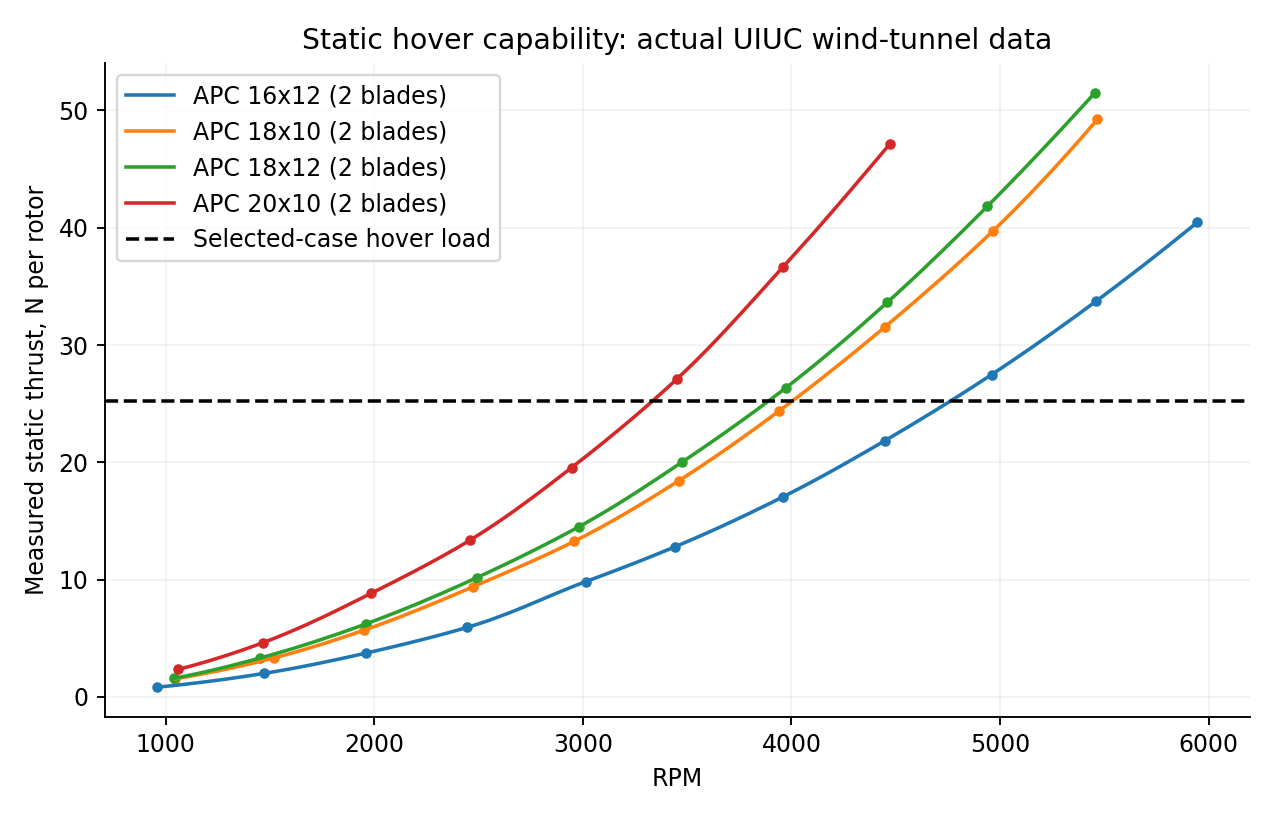
\includegraphics[width=.86\linewidth]{01_measured_hover_thrust.png}
\caption{Published UIUC static thrust data and the load for the illustrative takeoff mass. Smooth curves interpolate measured points within their recorded RPM bounds.}
\end{figure}
\begin{figure}[H]\centering
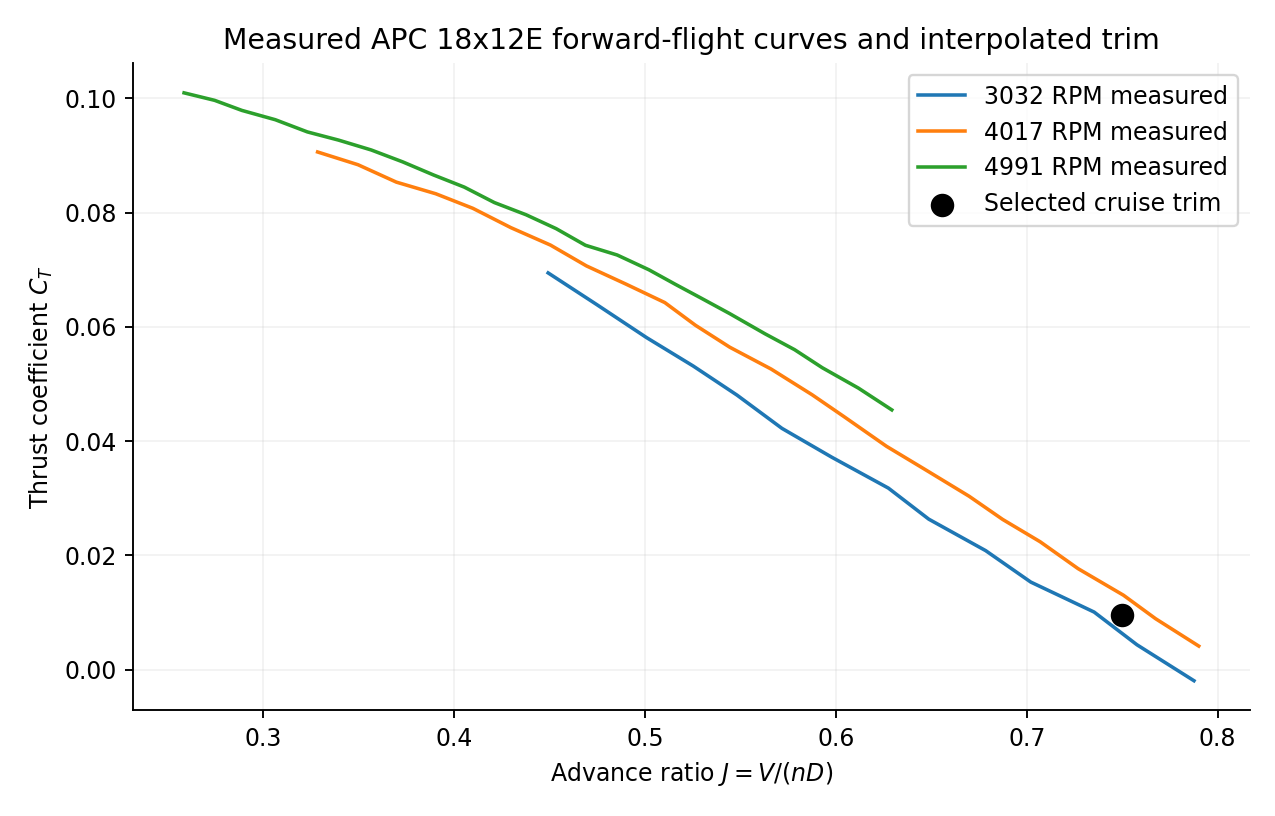
\includegraphics[width=.86\linewidth]{02_measured_cruise_ct.png}
\caption{Measured APC 18$\times$12E forward-flight thrust coefficients at recorded RPMs, and the interpolated 20-m/s cruise trim.}
\end{figure}
\begin{figure}[H]\centering
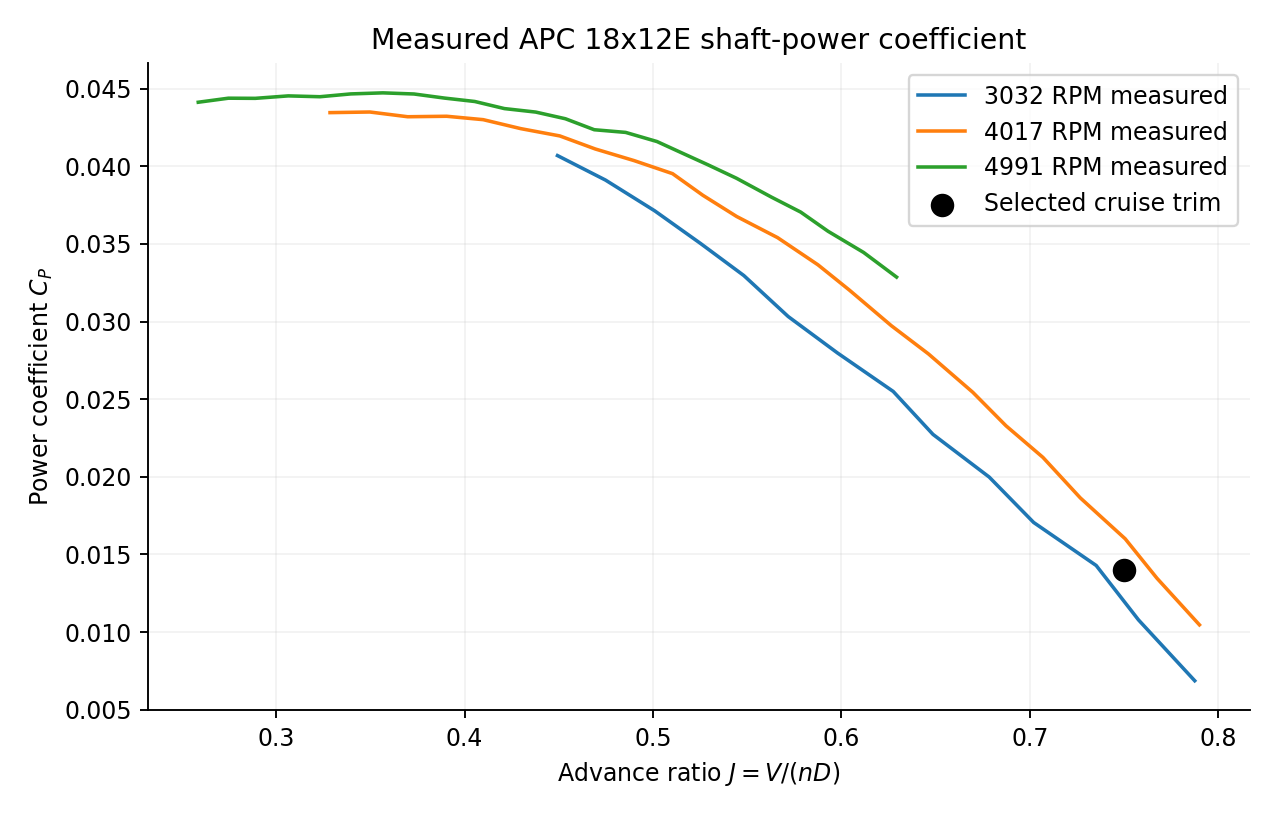
\includegraphics[width=.86\linewidth]{03_measured_cruise_cp.png}
\caption{Measured power coefficients for the same propeller, including the matched torque/power cruise operating point.}
\end{figure}

\subsection*{3.4 Numerical interpolation verification and parameter studies}
Withheld alternate measured rows were used to check interpolation rather than fit every point. Across the studied static curves, median holdout coefficient-error magnitudes normalized by the corresponding measured coefficient range were 5.17\% for $C_T$ and 6.59\% for $C_P$. For forward-flight curves, the analogous medians were 0.41\% and 0.59\%, respectively. These numbers represent \emph{interpolation accuracy within the same experimental campaign}, not an independently validated BEMT prediction at new blade geometry. Nominal rather than UIUC-measured diameters and differences between current product and historic test specimens remain error sources.

In a 25-case re-trim study, base aircraft mass was varied between 8.5 and 10.5 kg, and cruise drag between 5 and 9 N at fixed $20$-m/s cruise speed. Optimized rotor electrical energy varied from 237.8 to 319.7 Wh within the screened experimental domain. Increasing mass raises hover thrust and power; increasing cruise drag raises cruise shaft power and mission energy. The 18$\times$12E remains the measured-domain feasible candidate in the studied scenarios.
\begin{figure}[H]\centering
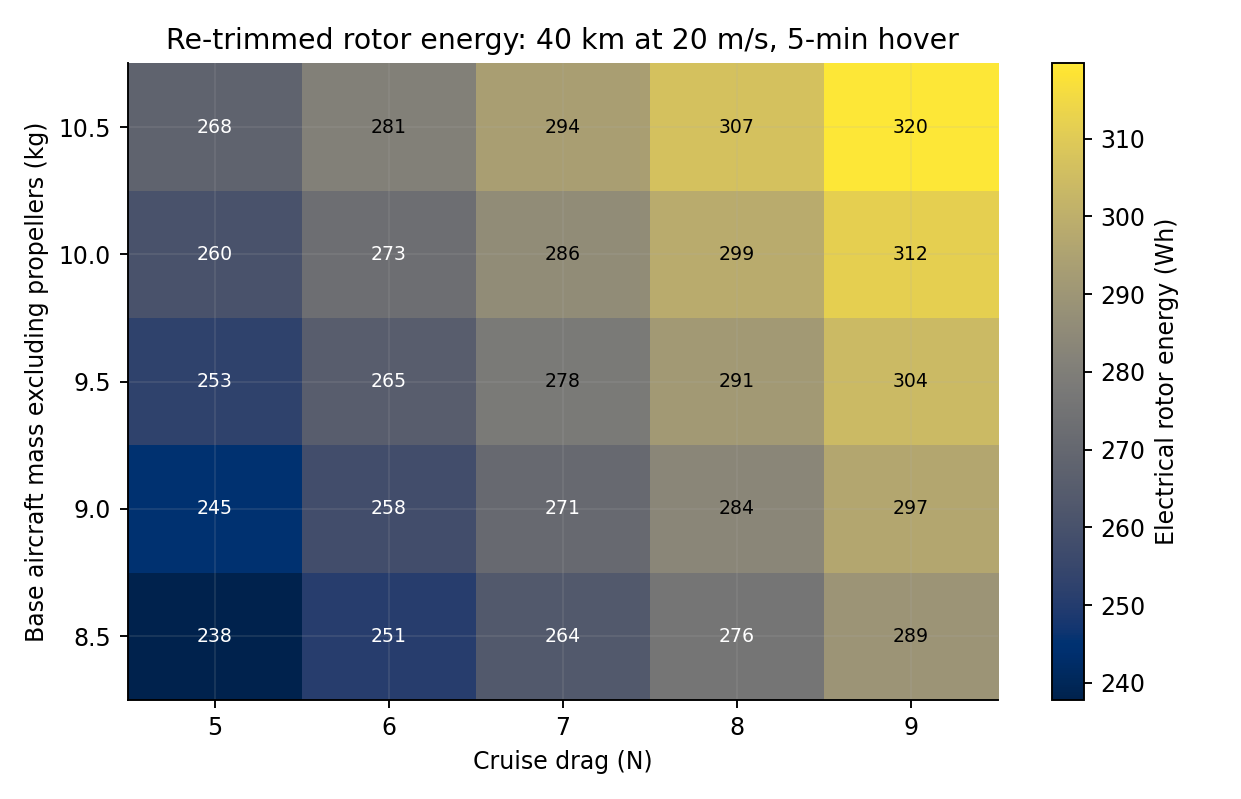
\includegraphics[width=.86\linewidth]{04_mass_drag_sensitivity.png}
\caption{Full re-trim sensitivity to the wing/system inputs; each cell solves hover and cruise thrust, and rejects unmeasured operating points.}
\end{figure}

A separate speed sweep at $\Delta V=0.25$ m/s admits experimentally bounded rotor trim only for approximately 16.75--23.5 m/s among the tested catalogue. The official 33.33-m/s requirement lies beyond the supported envelope. Reducing cruise speed increases flight time: at 20 m/s, 40 km requires 33.33 minutes, not the proposed 20 minutes.
\begin{figure}[H]\centering
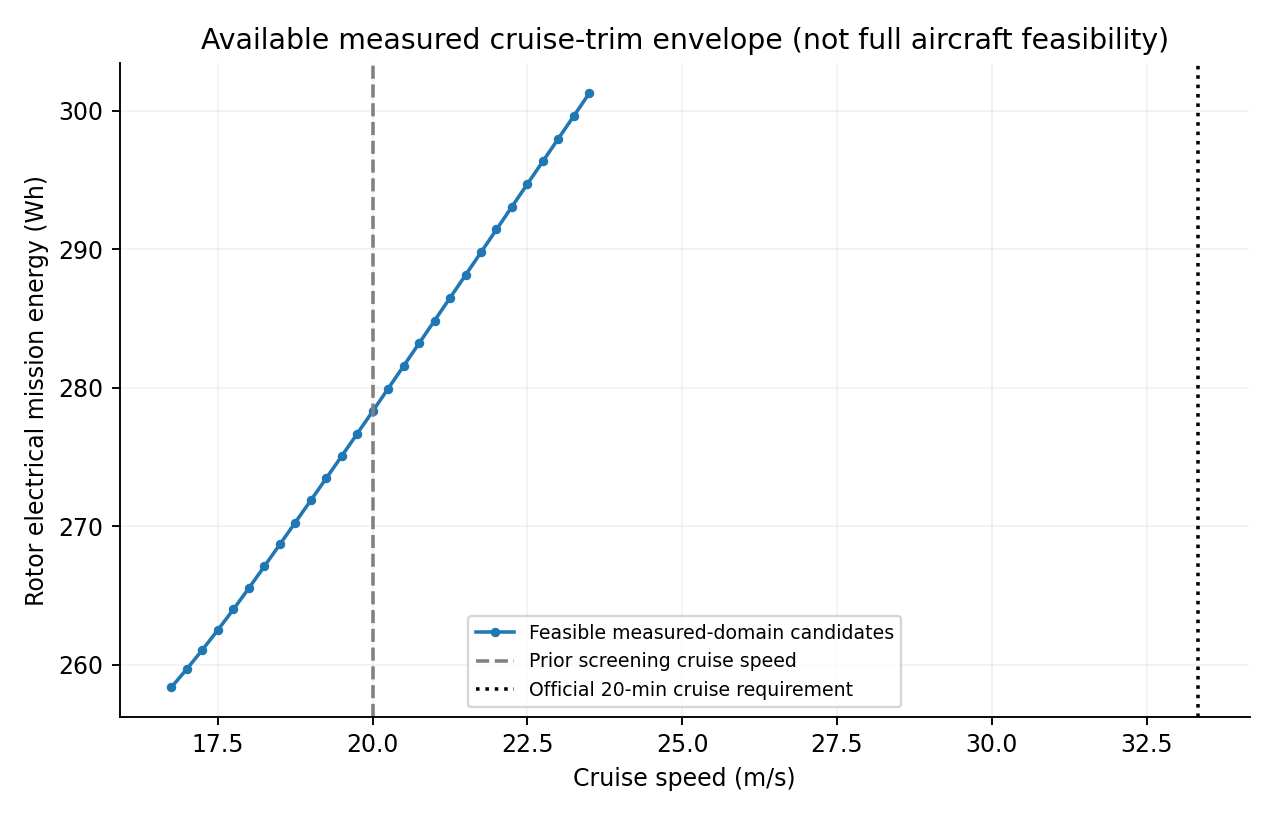
\includegraphics[width=.86\linewidth]{05_speed_energy_envelope.png}
\caption{Data-supported flight-speed/energy trade-off and the official mission requirement. Absence of a curve beyond the observed envelope denotes \emph{unsupported extrapolation}, not infinite energy.}
\end{figure}

A $\pm1\%$ perturbation to the nominal diameter input changes the calculated alternative mission energy from about 277.0 to 279.6 Wh after re-trimming; this tests a numerical input uncertainty, not an independently measured diameter correction. The candidate performance has not been structurally tested for the proposed tiltrotor installation.

\section*{4. LESSONS LEARNED AND DESIGN RECOMMENDATIONS}
First, a formally converged SLSQP solution is only as trustworthy as the forward model. The old constant-pitch, five-variable BEMT optimization permitted mixed negative/positive annular loading but clipped the negative contributions in the momentum update. Correcting the algorithm to use signed annular momentum equations causes the old cruise point to fail its low-induction admissibility test. The original three-blade 138.10-Wh result must therefore not be used to size motors or batteries or to claim an optimal blade count.

Second, a measured-data catalogue search yields more defensible engineering numbers but narrows the freedom of the design space. It can support a local selection from tested two-bladed configurations but cannot establish the best continuous chord, radius or blade pitch, nor exclude untested three- or four-bladed propellers. The APC 18$\times$12E is a conditional screening preference for a slower 20-m/s mission, not a universal global optimum. The 278.3-Wh rotor-only energy estimate should be updated when the wing's actual drag, actual propeller test diameters, motor/ESC map, and total aircraft mass are agreed.

Third, the official mission is a real design constraint. A 40-km sortie in 20 minutes requires a much faster operating point than the earlier screen. No candidate in the restricted tested catalogue can presently be qualified at this speed. Suitable future options include a documented high-pitch propeller family with forward-flight measurements at high advance ratio, revision of the 20-minute cruise requirement with team approval, or an aerodynamic propulsion architecture change. None should be presented as already demonstrated.

\section*{5. SYSTEM LEVEL CONSIDERATIONS}
The rotor subsystem sends Damian $N_r=4$, the propeller selected and its mass, the thrust/torque/RPM operating points, maximum electrical demand at reserve thrust, and the rotor component mission-energy budget. For the conditional 18$\times$12E alternative, hover/forward shaft torque is 0.631/0.185 N m per motor and corresponding speeds are 407/367 rad/s. Damian must use his voltage/current and efficiency model rather than treating the provisional 0.85 drive efficiency and the 2,400-W electrical ceiling as hardware facts. A flight-energy requirement of 278.3 Wh does not include avionics, transition and other system loads, nor battery reserve; nominal battery capacity must account for usable depth of discharge and additional loads.

Antoine must verify rotor mounting spacing, local wing clearance/download, cruise drag at each speed, and lift/transition requirements. The proposed $m_b=9.5$ kg is a scenario assumption that includes an unverified airframe, wing, battery, motor and payload ledger; it is \emph{not} a converged vehicle estimate. The propeller mass must not be counted twice, and the nacelle/tilt mechanism and motor masses belong in the coupled design ledger. A credible team MDO loop should update wing drag, propeller geometry, motor and battery mass, then total takeoff mass and hover load until consistent, including transition operation and an agreed cruise-speed requirement.

The current deliverable therefore supports a completed \emph{bounded rotor optimization investigation} with actual wind-tunnel performance and transparent limitations. The full system's original 20-minute, 40-km mission cannot yet be signed off from the current hardware tests; that is a documented engineering conclusion, not an omitted experiment.

\section*{References}
\begin{enumerate}
\item Dantsker, O. D., Caccamo, M., Deters, R. W., and Selig, M. S. (2022). ``Performance Testing of APC Electric Fixed-Blade UAV Propellers.'' \emph{AIAA Aviation Forum}, Paper 2022-4020. UIUC Propeller Database, Vol. 4. \url{https://m-selig.ae.illinois.edu/props/volume-4/propDB-volume-4.html}.
\item APC Propellers, product specification pages for 16$\times$12E, 18$\times$10E, 18$\times$12E and 20$\times$10E, including nominal pitch, diameter and mass. \url{https://www.apcprop.com/}.
\item MECH 559 Group 5 (2026). ``Energy optimization for VTOL tiltrotor hybrid UAV,'' project proposal and supervisor feedback.
\item MECH 559 (Fall 2026). \emph{Individual Project Report Guidelines}. Department of Mechanical Engineering, McGill University.
\item MECH 559 lectures L8--L9 (2026), nonlinear programming, regularity, active constraints, KKT conditions and sequential quadratic programming.
\end{enumerate}

\end{document}
